\begin{figure}[!t]
    \centering
    %\resizebox{\columnwidth}{!}{%
    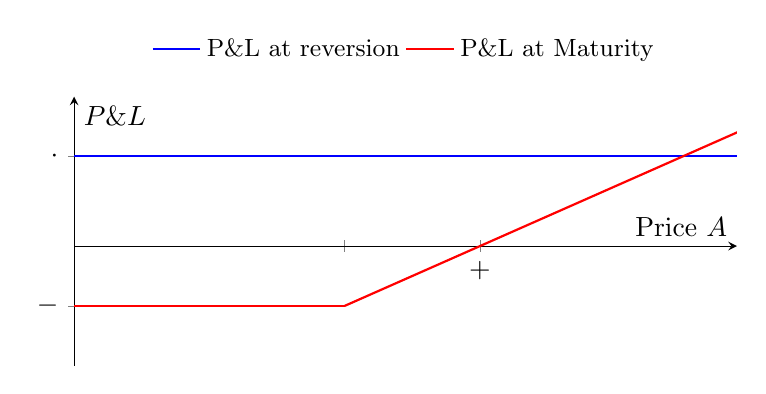
\begin{tikzpicture}[
      declare function={
        mypl(\x)= -1.25 + (\x>25) * (0.9*(\x-25));
      }
    ]
    \begin{axis}[
      xlabel={Price $A$},
      ylabel={$P\&L$},
      axis lines=middle,
      width=10cm,height=5cm,
      xmin=0,xmax=4.9,
      ymin=-2,ymax=2.5,
      ytick={-1,1.5}, 
      xtick={2, 3},
      xticklabels={$\strikePriceShort$, $\strikePriceShort+\premiumShort$},
      yticklabels={$-\premiumShort$, $\premiumShort \cdot \factorPrimitive$},
      legend style={
        draw=none,
        legend columns=-1,
        at={(0.5,1)},
        anchor=south,
        outer sep=1em,
        node font=\small,
      },
    ]
    
      %\addplot[blue,thick] {mypl(x)};
      \addplot[blue,thick] coordinates {(0,1.5) (5,1.5)};
      \addlegendentry{P\&L at reversion}
      %\addplot[pink, thick] {0.05*(x-20)^2-1.25};
      \addplot[red,thick] coordinates {(0,-1) (2,-1)};
      \addplot[red,thick] coordinates {(2,-1) (5,2)};
      \addlegendentry{P\&L at Maturity};
    \end{axis}
    \end{tikzpicture}
    \caption{Payoff \& Loss (P\&L) analysis for the Buyer $\buyerShort$ of the \financialPrimitive. In case of reversion, the payoff for the $\buyerShort$ is constant. In case of maturity, the payoff is equal to a traditional call option.}
    \label{figure:payoffCurve}
\end{figure}